\section{Local Certification And One-Transition Survival}
\label{sec:local-certification}

Complete-period growth becomes relevant to twin primes only after a theorem
places a surviving 2-gap inside an eligible square-safe window. This section
first proves what such a survivor certifies, then isolates the exact local
attrition conditions needed to retain one.

\subsection{Safe-Window 2-Gaps Certify Twin Primes}
\label{sec:safe-window-certify-twin-primes}

The square bound turns acceptance into primality. Any composite below $Q^2$
has a prime divisor below $Q$, but every such divisor has already been
installed as a filter. Therefore, for every prime future head $Q$ and every
accepted integer $n$ with $Q\le n\lt Q^2$ after all primes below $Q$ are
installed, a surviving accepted pair at distance $2$ is not merely a
putative pair; it is a twin-prime pair.

Let
\begin{equation*}
P_Q=\prod_{r\lt Q}r,
\end{equation*}

where $r$ ranges over primes. If
\begin{equation*}
Q\le n\lt Q^2,
\qquad
\gcd(n,P_Q)=1,
\end{equation*}

then $n$ is prime. Indeed, suppose that $n$ were composite. It has a prime
divisor $r\le\sqrt n$. The strict square bound gives
$r\le\sqrt n\lt Q$, so $r$ is one of the factors of $P_Q$. Consequently
$r\mid n$ and $r\mid P_Q$, contradicting $\gcd(n,P_Q)=1$:
\begin{equation*}
\begin{aligned}
n\text{ composite}
&\Longrightarrow
\exists r\text{ prime}:r\mid n\ \land\ r\le\sqrt n
&&[\text{Small Prime Divisor}]\\
&\Longrightarrow r\lt Q
&&[\text{Strict Bound }n\lt Q^2]\\
&\Longrightarrow r\mid P_Q
&&[\text{By Definition}]\\
&\Longrightarrow \gcd(n,P_Q)>1
&&[\text{Since }r\mid n]\\
&\Longrightarrow \bot.
&&[\text{Contradiction}]
\end{aligned}
\end{equation*}

Hence $n$ is prime. Applying this result independently to both endpoints gives
\begin{equation*}
\begin{aligned}
& Q\le x,\qquad x+2\lt Q^2,\qquad \gcd(x(x+2),P_Q)=1\\
&\Longrightarrow x\text{ and }x+2\text{ are prime}
\qquad\blacksquare\ \text{[Q.E.D.]}
\end{aligned}
\end{equation*}

The right-endpoint inequality must be strict: $Q^2$ is composite but has no
prime divisor below $Q$. The theorem certifies one eligible survivor; it does
not prove that any such survivor exists.

{\raggedright
The derivation above proves the theorem and its endpoint discipline.
\par}

\subsection{Isolation Of 2-Gaps After Filter 3}
\label{sec:two-gap-isolation}

After filter $3$, two 2-gaps cannot share an endpoint, for every sieve stage
whose modulus $M$ is divisible by $6$. This improves the sharp destruction
capacity of one later filter strike: for every later deletion of an accepted
value, removing one accepted value can destroy at most one existing 2-gap.

Suppose both $(x,x+2)$ and $(x+2,x+4)$ were accepted 2-gaps. The three values
$x,x+2,x+4$ occupy all three residue classes modulo $3$, so exactly one is
divisible by $3$. Because $3\mid M$, that value cannot be accepted. Thus
\begin{equation*}
\begin{aligned}
& (x,x+2)\text{ and }(x+2,x+4)\text{ both accepted}\\
&\Longrightarrow 3\nmid x,\ 3\nmid(x+2),\ 3\nmid(x+4)
&&[\text{Acceptance}]\\
&\Longrightarrow \bot
&&[\text{Complete Residue System Modulo }3].
\end{aligned}
\end{equation*}

Equivalently, parity and filter $3$ force every 2-gap start into one residue:
\begin{equation*}
\begin{aligned}
x,x+2\text{ accepted}
&\Longrightarrow x\equiv1\pmod2
&&[\text{Filter }2]\\
&\Longrightarrow x\equiv5\pmod6.
&&[\text{Filter }3;\ \text{CRT}]
\end{aligned}
\end{equation*}

Any destroyed 2-gap must contain a removed accepted value as an endpoint. A
value could belong to two 2-gaps only in the forbidden overlapping
configuration above. Let $N_{\text{destroyed}}$ be the number of destroyed
2-gaps and $N_{\text{removed}}$ the number of removed accepted values.
Therefore
\begin{equation*}
N_{\text{destroyed}}
\le
N_{\text{removed}}.
\end{equation*}
\begin{equation*}
\qquad\blacksquare\ \text{[Q.E.D.]}
\end{equation*}

Isolation limits destruction efficiency. It does not imply that a chosen
window contains a 2-gap before or after the filter.

The isolation argument above forces $x\equiv5\pmod6$: the smallest gap that
can separate two consecutive 2-gaps is therefore the classic prime-quadruplet
pattern $[2,4,2]$, a distance of exactly $4$, never less. The figure below
measures this directly on the same 200-stage generated dataset used in
Section~3: the average and maximum distance between consecutive 2-gaps
(summed runs, not individual raw gaps), per stage. The average grows steadily
($4\to{\sim}125$) while the maximum grows much faster (${\sim}1450$ by the
last stage), diverging further as the head grows --- but the average's floor
sits at exactly $4$ across every stage, never lower, matching the isolation
bound proved above rather than merely approximating it.

\begin{figure}[htbp]
\centering
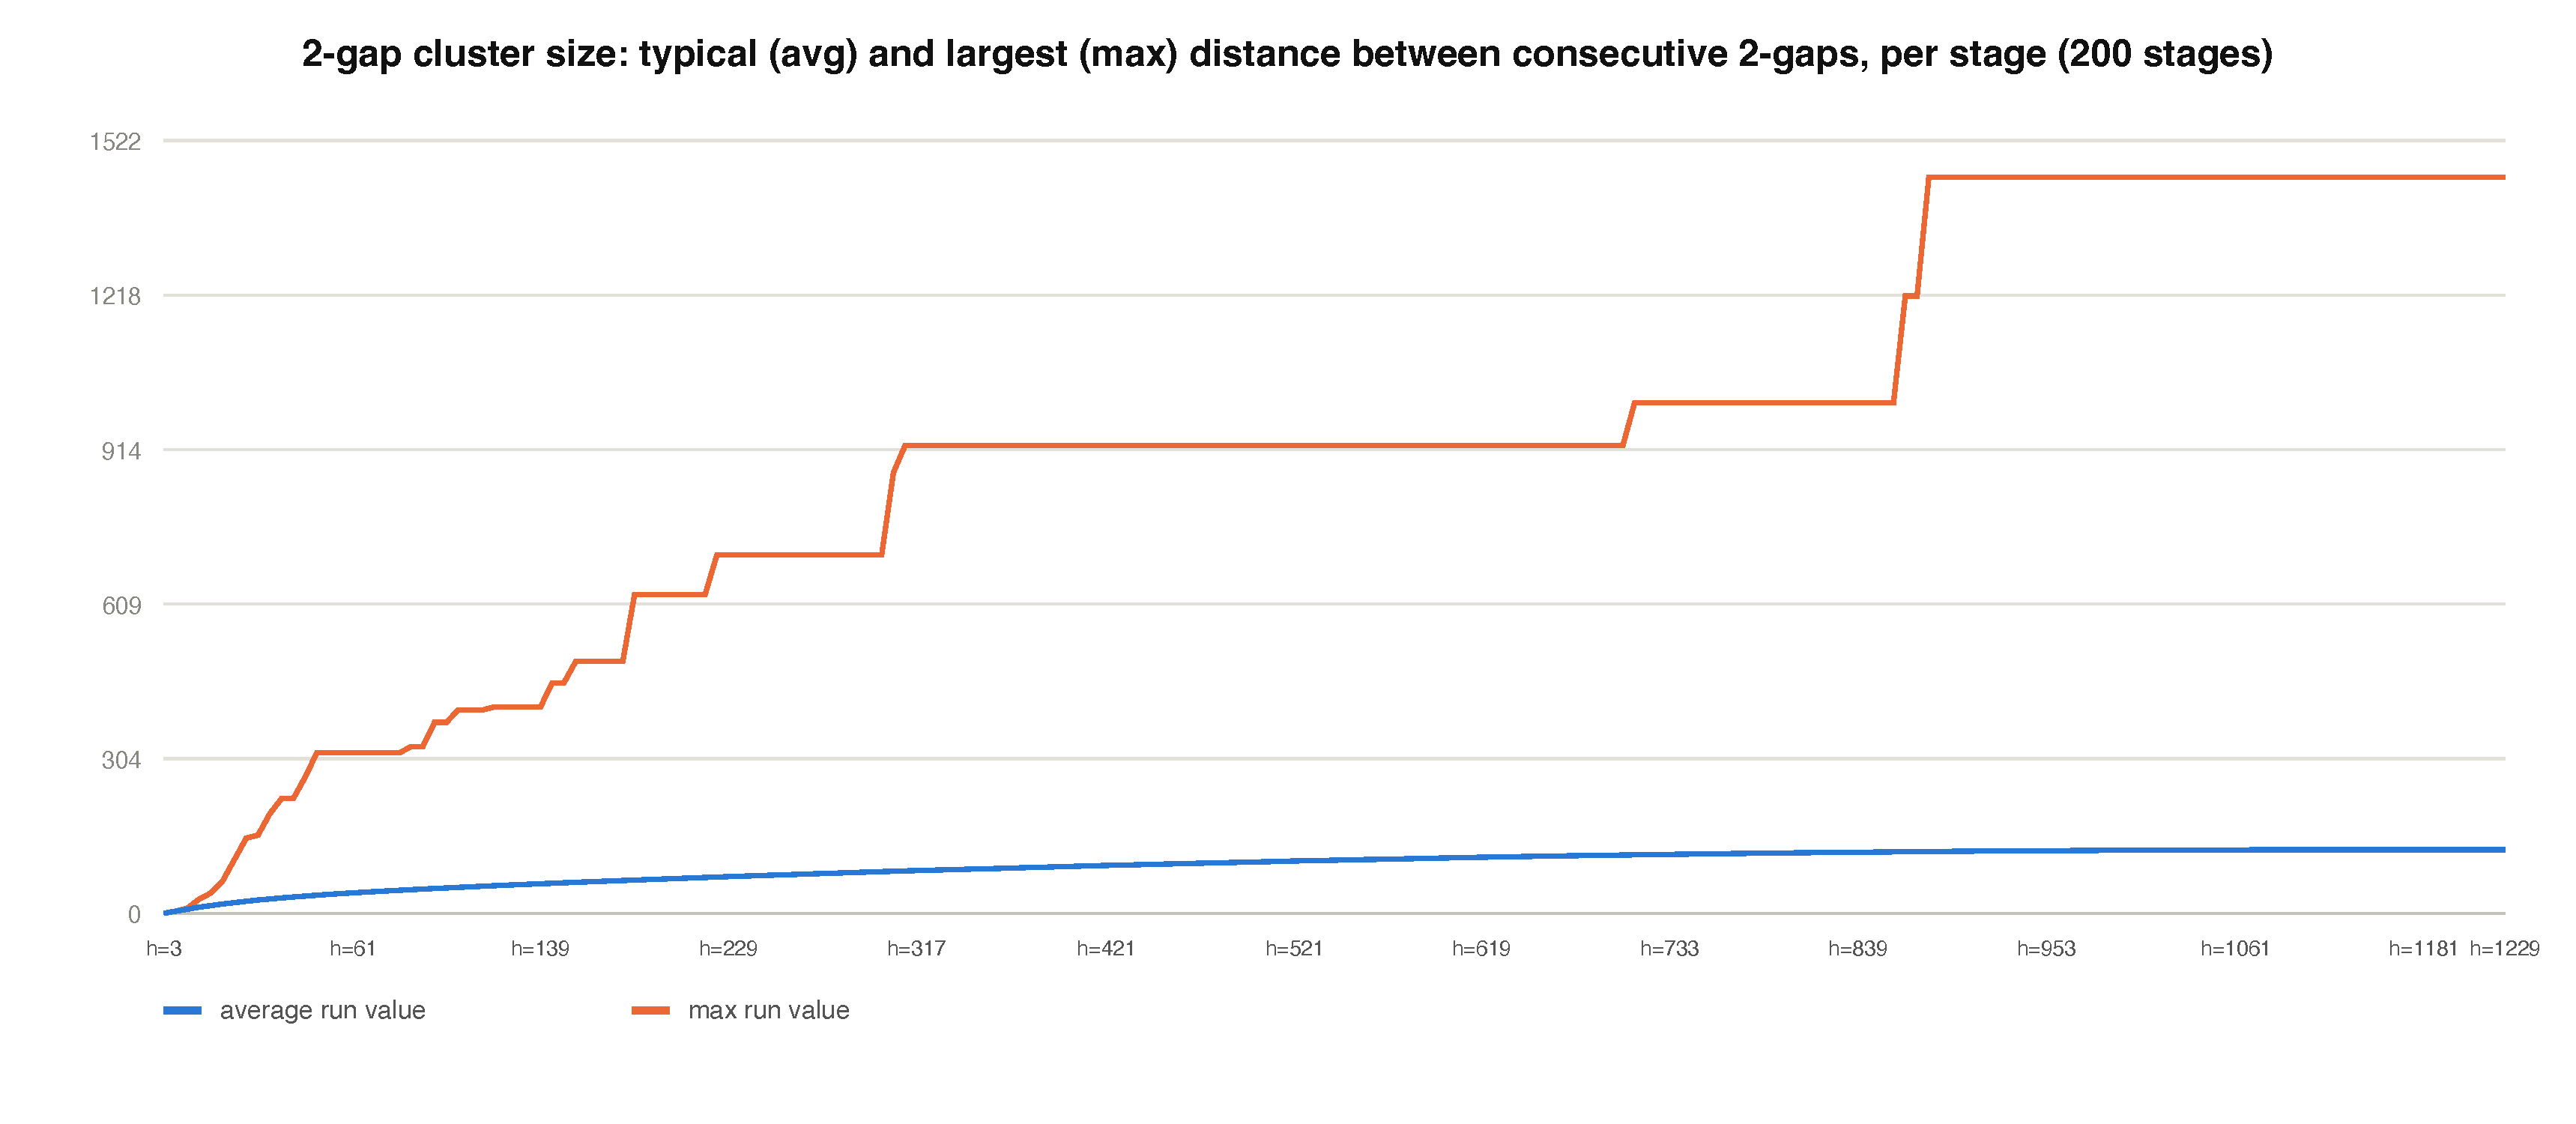
\includegraphics[width=\textwidth]{figures/gap-two-cluster-size.pdf}
\caption{Average and maximum distance between consecutive 2-gaps, per
stage; the average floor is exactly 4.}
\label{fig:gap-two-cluster-size}
\end{figure}

{\raggedright
The overlap argument above proves its filtering consequence. \par}

\subsection{Exact Accepted Local Filter Strikes}
\label{sec:accepted-local-strikes}

Counting every multiple of $r$ overstates local destruction because most
multiples have already been removed by smaller filters. For every incoming
prime $r\ge5$ and its next prime future head $Q$, the remaining multiples in
that square-safe window admit an exact prime-multiplier description, proved
here using Bertrand's postulate as an external dependency.

Let
\begin{equation*}
M_r=\prod_{s\lt r}s,
\qquad
K=\left\lfloor\frac{Q^2-1}{r}\right\rfloor,
\end{equation*}

where $s$ ranges over primes and $Q$ is the next prime after $r$. Before
filter $r$ is applied, the accepted multiples of $r$ in $[Q,Q^2)$ are exactly
\begin{equation*}
r\ell
\qquad\text{with }\ell\text{ prime and }r\le\ell\le K.
\end{equation*}

Consequently their number is
\begin{equation*}
A(r,Q)=\pi(K)-\pi(r-1).
\end{equation*}

Every multiple of $r$ in the window has the form $r\ell$ with
$2\le\ell\le K$, because Bertrand's postulate gives $r\lt Q\lt2r$. Since
$\gcd(r,M_r)=1$, this value survived the earlier filters exactly when
$\gcd(\ell,M_r)=1$.

Bertrand's bound also gives
\begin{equation*}
\begin{aligned}
K
&\lt\frac{Q^2}{r}
&&[\text{By Definition Of }K]\\
&\lt4r
&&[\text{Bertrand: }Q\lt2r]\\
&\le r^2.
&&[\text{Since }r\ge5]
\end{aligned}
\end{equation*}

If an accepted multiplier $\ell\lt K+1\le r^2$ were composite, its least prime
divisor would be at most $\sqrt\ell\lt r$ and would divide $M_r$, contradicting
$\gcd(\ell,M_r)=1$. Thus every accepted multiplier is prime and at least $r$.
Conversely, every prime $\ell\ge r$ is coprime to $M_r$. Therefore
\begin{equation*}
\begin{aligned}
& \#\{n\in[Q,Q^2):r\mid n,\ \gcd(n,M_r)=1\}\\
&=\#\{\ell:r\le\ell\le K,\ \ell\text{ prime}\}
&&[\text{Accepted Multiplier Characterization}]\\
&=\pi(K)-\pi(r-1)
&&[\text{Prime-Counting Definition}]\\
&=A(r,Q).
&&\blacksquare\ \text{[Q.E.D.]}
\end{aligned}
\end{equation*}

This is the exact count of accepted values struck by filter $r$ in the stated
window. A struck value need not be a 2-gap endpoint, so $A(r,Q)$ is only an
upper bound on the number of destroyed local 2-gaps.

{\raggedright
The derivation above proves the exact characterization, including its Bertrand
dependency. \par}

\subsection{Sharp Local 2-Gap Survival Threshold}
\label{sec:sharp-local-survival-threshold}

The proved theorem is the conditional implication below; its local-abundance
antecedent remains open. It holds for every incoming prime $r\ge5$, its next
prime future head $Q$, and the single transition that installs filter $r$,
over pre-filter and post-filter 2-gap starts whose two endpoints remain
inside one eligible square-safe window.

The exact accepted-strike count becomes a sharp deterministic survival test.
If the eligible window initially contains more 2-gaps than filter $r$ has
accepted values to remove, endpoint isolation forces at least one gap to
survive.

Let $G_{\mathrm{local}}(r,Q)$ count the pre-filter 2-gaps $(x,x+2)$ satisfying
\begin{equation*}
Q\le x,
\qquad
x+2\lt Q^2,
\end{equation*}

and let $G_{\mathrm{surviving}}(r,Q)$ count those still present after filter
$r$. With
\begin{equation*}
K=\left\lfloor\frac{Q^2-1}{r}\right\rfloor,
\qquad
A(r,Q)=\pi(K)-\pi(r-1),
\end{equation*}

let $G_{\mathrm{destroyed}}(r,Q)$ count the destroyed eligible 2-gaps. The
2-gap isolation and accepted local strikes properties give
\begin{equation*}
\begin{aligned}
G_{\mathrm{destroyed}}(r,Q)
&\le\#\{\text{accepted values struck in }[Q,Q^2)\}
&&[\text{2-Gap Isolation}]\\
&=A(r,Q).
&&[\text{Accepted Local Strikes}]
\end{aligned}
\end{equation*}

Therefore
\begin{equation*}
\begin{aligned}
G_{\mathrm{surviving}}(r,Q)
&=G_{\mathrm{local}}(r,Q)
  -G_{\mathrm{destroyed}}(r,Q)
&&[\text{Population Accounting}]\\
&\ge G_{\mathrm{local}}(r,Q)-A(r,Q).
&&[\text{Substitution}]
\end{aligned}
\end{equation*}

Both counts are integers, so
\begin{equation*}
G_{\mathrm{local}}(r,Q)>A(r,Q)
\Longrightarrow
G_{\mathrm{surviving}}(r,Q)>0
\qquad\blacksquare\ \text{[Integer Positivity; Q.E.D.]}
\end{equation*}

Equivalently, $A(r,Q)+1$ eligible pre-filter gaps suffice. The theorem does
not prove this local-abundance antecedent. Iterating it through later filters
would require a fresh eligible population bound at every transition.

{\raggedright
The derivation above proves the conditional theorem and its exact boundary.
\par}

\subsection*{Local Harmful-Excess Notation}
\label{sec:local-harmful-excess-notation}

Let $Q$ be a future prime head and define the eligible start window
\begin{equation*}
W_Q=\{x\in\mathbb{Z}:Q\le x\ \land\ x+2\lt Q^2\}.
\end{equation*}

For a fixed filter $r$, let $K_r(I)$ count the incoming 2-gap starts in an
interval $I$ destroyed because $r$ divides one endpoint. If $N_r(I)$ is the
incoming population, define its centered harmful excess by
\begin{equation*}
b_r(I)=K_r(I)-\frac{2N_r(I)}r.
\end{equation*}

The density term $2N_r(I)/r$ is not itself an upper bound. The sign and size
of $b_r(I)$ encode the interval-order information discarded by separate
capacity estimates.
